%% -*- coding: utf-8-unix -*-
%#!ptex2pdf -u -l -ot "-kanji=utf8 -synctex=1" -od "-f ipaex.map -p a4" oop
%#BIBTEX upbibtex oop
%#MAKEINDEX mendex -U oop
%#LPR "C:/w32tex/SumatraPDFPortable/SumatraPDFPortable.exe" oop.pdf
% -----------------------------------------------------------------------------------
\documentclass[uplatex,a4j,11pt]{jsarticle}
%\documentclass[a4j,11pt]{jarticle}
\usepackage{amsmath,amsthm,amssymb}
\usepackage[dvipdfmx]{graphicx}
%\usepackage[dviout]{graphicx}
\usepackage[dvipdfmx,%
 bookmarks=true,%
 bookmarksnumbered=true,%
 colorlinks=true,%
 linkbordercolor={0 0 0},%	color of border around links	RGB値 1 0 0
 linkcolor=black,%	color of links	red
 urlcolor=blue,
 setpagesize=false,%
 pdftitle={オブジェクト指向の考え方},%
 pdfauthor={清水俊一},%
 pdfsubject={オブジェクト指向の考え方},%
 pdfkeywords={regexp; LaTeX; search; replace;}]{hyperref}
\usepackage{pxjahyper}
\usepackage{here}

%% ページ高さ
\setlength{\textheight}{\paperheight}
\setlength{\topmargin}{-1in}
\addtolength{\topmargin}{35truemm}% 上の余白
\setlength{\headheight}{0truemm}
\setlength{\headsep}{0truemm}
\setlength{\footskip}{10truemm}
\addtolength{\textheight}{-61truemm}% -(上の余白+下の余白)
%% ページ幅
\setlength{\textwidth}{\paperwidth}
\setlength{\oddsidemargin}{-1in}
\addtolength{\oddsidemargin}{26truemm}% 左の余白
\setlength{\marginparsep}{0in}
\setlength{\marginparwidth}{0in}
\addtolength{\textwidth}{-52truemm}% -(左の余白+右の余白)

\usepackage{amsmath}
\usepackage{framed}
\usepackage[usenames]{color}

\newcommand{\g}[1]{\mathbf {#1}}

\newenvironment{shadedf}{%
  \def\FrameCommand{\fcolorbox{black}{shadecolor}}%
  \MakeFramed {\advance\hsize-\width \FrameRestore}%
  }%
{\endMakeFramed}

\newenvironment{shadedfw}{%
  \def\FrameCommand{\fcolorbox{white}{shadecolor}}%
  \MakeFramed {\advance\hsize-\width \FrameRestore}%
  }%
{\endMakeFramed}

\kanjiskip=.1zw plus 3pt minus 3pt % 全角文字間
\xkanjiskip=.1zw plus 3pt minus 3pt % 全角半角文字間
\def\baselinestrech{1.2} % 行間を少し開く
\renewcommand{\baselinestretch}{1.08}
% 丸数字
\def\MARU#1{\leavevmode \setbox0\hbox{$\bigcirc$}%
\copy0\kern-\wd0 \hbox to\wd0{\hfil{{\footnotesize #1}}\hfil}}

\author{平成28年度 情報論理}
\title{オブジェクト指向の考え方}
\date{}
%% ------------------------------------------------------------
\usepackage{ascmac}	% required for `\shadebox' (yatex added)
\begin{document}

\maketitle
\pagestyle{plain}

% 目次の表示
\tableofcontents

\newpage
\def\baselinestretch{.9}\selectfont
%% ------------------------------------------------------------
\section{図形を描く}

processing を使って図形を描きながら、考え方を確かめる。

{\bfseries ※ プログラムは論理の組み立てである}

以下が processing のスケルトン。
エディタに書いて実行(Ctrl + R)すると 800 * 600 の大きさのカンバスが現
れる。

   \begin{quote}
	\begin{minipage}{\linewidth}
	 \begin{shadebox}
      \def\baselinestretch{.8}\selectfont
      \small
      \begin{verbatim}

/*
 * prim00.pde
 * 図形を描く1
 */

// クラス変数 クラス内の全メソッドで使える
int width = 800;
int height = 600;

/********************************************************
 * 最初に1回だけ動く関数(メソッド)
 *   おもに初期設定に使う
 ********************************************************/
% P3 ではこうする
%void settings(){
%  size(width,height);    // 描画領域
%}

void setup(){
  size(width,height);    // 描画領域
  frameRate(20);    // 1秒間に描写するフレーム数
  smooth();
}

/********************************************
 * frameRate に応じて何度も動く(ループする)
 * 座標などを変えると絵を動かすことができる
 ********************************************/
void draw() {
  background(130, 160, 180);    // 背景の色 (Red, Green, Blue)
}
      \end{verbatim}
	 \end{shadebox} 
	 \end{minipage}
	\end{quote}

\begin{itemize}
 \item 
       \href{https://www.processing.org/reference/}{Processing Reference}
       : https://www.processing.org/reference/
\end{itemize}


\subsection{四角を描く}

    \begin{quote}
	\begin{minipage}{\linewidth}
	 \begin{shadebox}
      \def\baselinestretch{.8}\selectfont
      \small
      \begin{verbatim}

    // 四角を描く rect(x, y, w, h)
    // x, y : 座標
    // w, h : 幅, 高さ
    rect(0, 0, 200, 100);  // processing の組込関数
      \end{verbatim}
	 \end{shadebox} 
	 \end{minipage}
	\end{quote}

    \begin{itemize}
     \item 
           描画領域を確認せよ
     \item 
           座標の位置を確認せよ
    \end{itemize}


\subsection{円を描く}

    \begin{quote}
	\begin{minipage}{\linewidth}
	 \begin{shadebox}
      \def\baselinestretch{.8}\selectfont
      \small
      \begin{verbatim}

    // 円を描く ellipse(x, y, w, h)
    // x, y : 座標
    // w, h : 幅, 高さ
    ellipse(0, 0, 200, 100);
      \end{verbatim}
	 \end{shadebox} 
	 \end{minipage}
	\end{quote}

    \begin{itemize}
     \item 「四角を描く rect(x, y, w, h)」と違うのは?
    \end{itemize}

\subsection{四角と円の位置を合わせる}

次の図 \ref{145345_19Jul14} のようにするにはどうする?

\begin{figure}[htbp]
  \begin{center}
   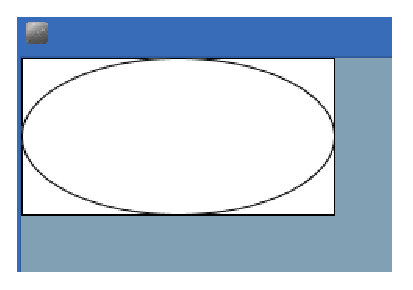
\includegraphics{zu1.eps}
   \caption{}
   \label{145345_19Jul14}
  \end{center}
\end{figure}

\href{prim00.txt}{コード例}


\subsubsection{ポイント}
\begin{itemize}
 \item \verb|void draw() {}| の中にデータを直打ちするのはどうか?
       \begin{itemize}
        \item \verb| rect(0, 0, 200, 100);|
        \item \verb| ellipse(0, 0, 200, 100);|
       \end{itemize}
 \item たとえば四角の大きさが変わったとき、それに合わせて円の大きさを変
       更するには何個数字を書き換えることになる?
 \item データ(数値)を「変数」に置き換えて設計できるのは{\bfseries 抽象
       化}の能力
\end{itemize}

\subsection{四角と円の共通点と相違点}

\begin{itemize}
 \item 共通点
       \vspace*{3zw}
       %変数の種類と数が同じ x,y,w,h
 \item 相違点
       \vspace*{3zw}
       % x,y の位置 四角が左上隅、円が中心の座標
\end{itemize}

{\bfseries ※ あとで「クラス」を作るときに参照する}

\subsection{図形を動かす}

\begin{itemize}
 \item x の値を変えれば x軸方向に動く\\
       \hspace{2zw} x += 1;

 \item y の値を変えれば y軸方向に動く\\
       \hspace{2zw} y += 1;

 \item x, y 両方の値を変えれば斜め方向に動く
\end{itemize}

{\bfseries ※ 問題はそのコードを「どこに」「どう」書くか}

\href{prim01.txt}{コード例}

\begin{itemize}
 \item 「\verb|x += moveX;  y += moveY;|」 の行を \\
       「\verb|// 円を描く ellipse(x, y, w, h) |」
       の前に移動したら、どうなると思う?
       \begin{itemize}
        \item 四角は動かずに円だけが動いていくだろうか?
       \end{itemize}
\end{itemize}

\subsection{たくさん動かす}
\label{たくさん動かす}

{\bfseries ※ それぞれの図形がそれぞれ勝手に動くようにするには?}

\begin{figure}[htbp]
  \begin{center}
   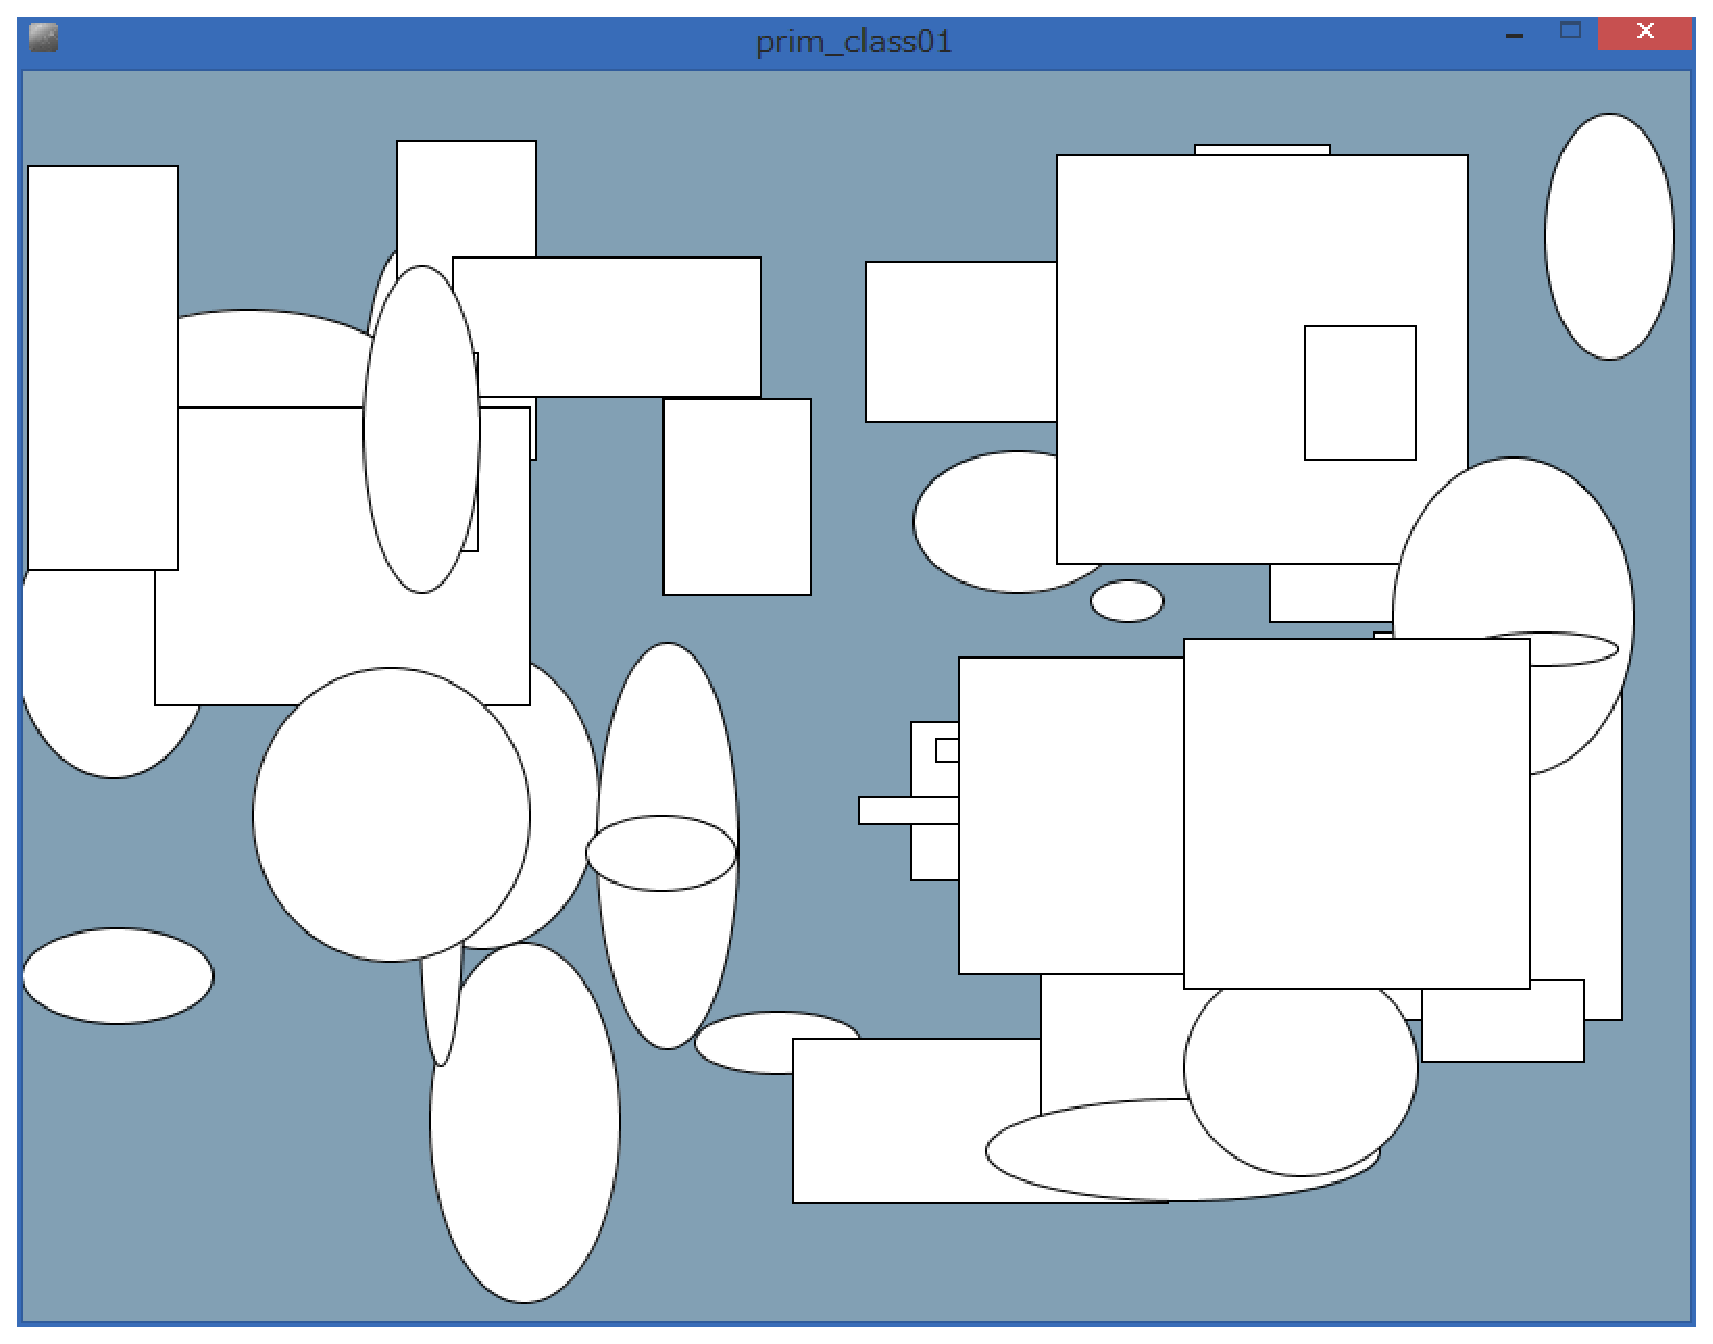
\includegraphics[width=.5\paperwidth]{zu2.eps}
   \caption{}
   \label{070938_20Jul14}
  \end{center}
\end{figure}

\begin{quotation}
 いきなり四角と円の両方に対処するのは無理があるので、とりあえず四角だけ
 を複数作ってみよう。

 次のようにして、円の描画部分をコメントアウトしておく。

    \begin{quote}
	\begin{minipage}{\linewidth}
	 \begin{shadebox}
      \def\baselinestretch{.8}\selectfont
      \small
      \begin{verbatim}

  // 円を描く ellipse(x, y, w, h)
  // x, y : 座標 円の中心の位置
  // w, h : 幅, 高さ
//  ellipse(x + w / 2, y + h /2, w, h);
      \end{verbatim}
	 \end{shadebox} 
	 \end{minipage}
	\end{quote}
\end{quotation}

描く図形ごとに x, y, w, h,moveX, moveY は異なるから、これらを「配列」に
作っておく。
\label{174855_21Jul14}

    \begin{quote}
	\begin{minipage}{\linewidth}
	 \begin{shadebox}
      \def\baselinestretch{.8}\selectfont
      \small
      \begin{verbatim}

float x[] = new float[MAX];
float y[] = new float[MAX];
float w[] = new float[MAX];
float h[] = new float[MAX];
float moveX[] = new float[MAX];
float moveY[] = new float[MAX];
      \end{verbatim}
	 \end{shadebox} 
	 \end{minipage}
	\end{quote}


図形をたくさん描くには for 文でループさせればよい。

    \begin{quote}
	\begin{minipage}{\linewidth}
	 \begin{shadebox}
      \def\baselinestretch{.8}\selectfont
      \small
      \begin{verbatim}

  for(int i=0; i<MAX; i++){
    rect(x[i], y[i], w[i], h[i]);  // processing の組込関数
    // 移動量
    x[i] += moveX[i];  y[i] += moveY[i];
  }
      \end{verbatim}
	 \end{shadebox} 
	 \end{minipage}
	\end{quote}

    この場合 for 文の中でカウントしている「 i 」が、描画する図形の番号を
    表している。
    \begin{itemize}
     \item 図形[0] の座標が \verb|x[0], y[0]|、大きさが \verb|w[0], h[0]|\\
           X軸方向の移動量が \verb|moveX[0]|、 Y軸方向の移動量が \verb|moveY[0]|

     \item 図形[1] の座標が \verb|x[1], y[1]|、大きさが \verb|w[1], h[1]|\\
           X軸方向の移動量が \verb|moveX[1]|、 Y軸方向の移動量が \verb|moveY[1]|
     \item 図形[2] の座標が x[2], y[2]、大きさが w[2], h[2]\\
           X軸方向の移動量が \verb|moveX[2]|、 Y軸方向の移動量が
           \verb|moveY[2]|
    \end{itemize}



    \verb| random() |関数を使うと乱数を発生させられる。

    \begin{quote}
	\begin{minipage}{\linewidth}
%	 \begin{shadebox}
      \def\baselinestretch{.8}\selectfont
      \small
      \begin{verbatim}

        random(100);     // 0 から 100 までの数値をランダムに発生
        random(10, 20);  // 10 から 20 までの数値をランダムに発生

        random(width);  // width は描画領域の横幅を表す
        random(height); // height は描画領域の横幅を表す
      \end{verbatim}
%	 \end{shadebox} 
	 \end{minipage}
	\end{quote}

    これを使ってすべてのデータ(変数)をランダムに設定できる。

    \begin{quote}
	\begin{minipage}{\linewidth}
	 \begin{shadebox}
      \def\baselinestretch{.8}\selectfont
      \small
      \begin{verbatim}

  //変数初期化
  for(int i=0; i<MAX; i++){
    x[i] = random(width); y[i] = random(height);
    w[i] = random(10,200); h[i] = random(10,200);
    moveX[i] = random(1,5); moveY[i] = random(1,5);
  }
      \end{verbatim}
	 \end{shadebox} 
	 \end{minipage}
	\end{quote}

    おまけ。

    このままだとせっかく描画した図形がカンバスの外に出ていったままいなく
    なってしまうので、次のようにしてみよう。
    よく読めば何をやっているかわかるね?
    
    \begin{quote}
	\begin{minipage}{\linewidth}
	 \begin{shadebox}
      \def\baselinestretch{.8}\selectfont
      \small
      \begin{verbatim}

    // 跳ね返り
    if(x[i] < 0 || x[i] + w[i] > width) moveX[i] *= -1;
    if(y[i] < 0 || y[i] + h[i] > height) moveY[i] *= -1;
      \end{verbatim}
	 \end{shadebox} 
	 \end{minipage}
	\end{quote}

\href{prim020.txt}{コード例}

    ただ、これで描画するとおかしな動きをする奴がたまに出現する。実行して
    みるとわかる。なぜおかしな動きになるか、理由を考えて対処してみて。
\href{prim02.txt}{コード例}

\medskip
{\bfseries ※ 四角はこれでいいとして、円を同様にたくさん作って動かす
にはどうする?}

\begin{quote}
 円は円で、四角とは別に操作するわけだから、新たに円用の変数配列を
 作ることになるか。たとえば \verb|x[i], y[i], w[i], h[i]| にしても
\begin{itemize}
 \item 四角用 : \verb|bx[i], by[i], bw[i], bh[i]| (b は box の略)
 \item 円用 : \verb|cx[i], cy[i], cw[i], ch[i]| (c は circle の略)
\end{itemize}
のようにするかな。

 配列は同じタイプの変数を一手に操作するには便利だが、これだけ多種類のも
 のを要素番号で区別しながらコーディングするのは頭が痛いよね。

\end{quote}

\newpage

\section{オブジェクト指向}

\subsection{処理中心からオブジェクト中心へ}

ここまでの「目次」をリストアップしてみると次のようになる。

 \begin{itemize}
  \item 図形を{\bfseries 描く}
        \begin{itemize}
         \item 四角を{\bfseries 描く}
         \item 円を{\bfseries 描く}
         \item 図形を{\bfseries 動かす}
         \item たくさん{\bfseries 動かす}
        \end{itemize}
 \end{itemize}

作業は「動き(動詞)」で表現される。
つまり、作業の中心は「処理」を手がかりに進めてきたことがわかる。

処理中心の考え方は、システムが「何を{\bfseries する}か」から考えて全
体を組み立てるものだ。システムの動きが「確定」していればとてもわかりやす
いし、コードも書きやすくなる。

しかし、処理を中心に組み立てると、たくさん存在する図形が「それぞれ勝手に
動くようにする」ような処理はとても煩雑になる。
(たとえばそれぞれの図形の座標を、全て区別するために膨大な変数の判別をし
なくてはならない)
「処理」を正確に稼働させるために、天空にコントロールセンターを置いて、そ
こからトップダウン式に全体を制御しているようなものだ。

壁にぶつかって跳ね返る処理を追加したが、配列の要素番号(index)で区別し
ながら個々の図形に動きを施しているのがわかるだろう。

%跳ね返るのが「動かない」壁だから、まだ簡単だが、もし、
%図形どうしがぶつかって跳ね返るようにするにはどうする?
%処理中心だと配列の要素でしか区別できないから、とんでもない数の条件分岐が
%発生しそうだ。

\begin{quotation}
 繰り返すが、処理中心の考え方は、これはこれで有効な考え方である。

 そのシステムが「どういう動きをするか」を基準にして分析する考え方だから、
 処理の仕様がかっちり定まっていて大きな改変がないようなシステムなら、分析
 も確定できるし、処理も書きやすい。
 (たとえば、会社の会計処理とか)

 だが、時代は変化が大きく常に新しいトレンドが生まれ、それに対応せざるをえ
 なくなっている。
\end{quotation}

「処理」のまとまりを単位として切り出し(これを「モジュール」と呼ぶ)、そ
れを構造的に組み上げることを{\bfseries 「構造化プログラミング」}という。
「構造化プログラミング」の基本構造は
\begin{itemize}
 \item 順次処理
 \item 条件分岐
 \item 繰り返し処理
\end{itemize}
だ。この3つの処理を組み立てながらプログラミングする。
構造化プログラミングを実現する構造化言語の代表格が「C言語」である。

\subsection{クラスという考え方}

動くものに目を向けるのではなく、その前に「存在」するもの(これを「オブジェ
クト」と呼ぶ)を見る。「モノ」中心に見るということ。

また、「動き」ではなく「データ」を中心に見る、ということもできる。
先の「\ref{たくさん動かす} たくさん動かす」処理でも、結局はそれ
ぞれの図形が持つ(\verb|x[i], y[i], w[i], h[i]|)の変化が動きをもたらしていた。

つまり、
{\bfseries 
「動き」をつけるために「データ」を変化させた、と考えるのではなく、
「データ」の変化が「動き」をつけた
}
、と考えるわけ。

すると、考え方が「動詞」から「名詞」中心になるのがわかるかな?
そう、「クラス」はそのシステムを分析したときに{\bfseries 名詞}として表現
されるものである。

次の仕様から「クラス」になり得る名詞を抜き出しなさい。

    \begin{quote}
	\begin{minipage}{\linewidth}
	 \begin{shadebox}
      \def\baselinestretch{.8}\selectfont
      \small
      \begin{verbatim}

        四角形は座標と大きさを持つ。
        rect(x, y, w, h) が四角形を描く。
        円は座標と大きさを持つ。
        ellipse(x, y, w, h) が円を描く。
      \end{verbatim}
	 \end{shadebox} 
	 \end{minipage}
	\end{quote}

    {\bfseries ※ 名詞がすべてクラスになるわけではないことに注意}

    {\bfseries ※ クラスが持つデータも名詞で表現される(「属性」と呼ぶ)}

\subsection{クラスは「型」}

有名な比喩を挙げておく。

クラスはクッキーを作る時の「型」と同じだ。
小麦粉を練った生地から型抜きをするための「型枠」(星形とかハート形とか)
のことだ。
この「型枠」は出来上がる形を規定しているが、実際に食べられない。あくまで
も、クッキー(オブジェクト)の形を定義しているだけ。

この「型枠」からそれぞれの形に抜き出されたものが、実際に食べられるクッキー
になる。これを{\bfseries 「インスタンス」(実体)}という。

また、プログラム的に見ても、いわゆる変数の「型」と同じようにクラスを扱う。
次の例は「クッキー」クラスの変数 \verb|cookie| を宣言して、同時にインス
タンスも作っている。
上の行の「\verb|int i;|」と似た形になっている
のがわかるだろう。

    \begin{quote}
	\begin{minipage}{\linewidth}
	 \begin{shadebox}
      \def\baselinestretch{.8}\selectfont
      \small
      \begin{verbatim}

        int i;          // int 型の変数 i を宣言
        Cookie cookie;  // Cookie 型の変数 cookie を宣言
        cookie = new Cookie();  // new 演算子はインスタンスを作る
      \end{verbatim}
	 \end{shadebox} 
	 \end{minipage}
	\end{quote}


\subsection{属性(データメンバ・メンバ変数・フィールド)}

クラスは「属性」を持つ。属性は「そのクラスの成り立ちを示すデータ」
\cite{Tucker}である。

例えば、「生徒」クラスならば、「学年」「組」「出席番号」「名前」などの属
性を持っている。上の「四角形」クラスなら「座標(x,y)」「大きさ(w,h)」
がそれにあたる。

属性は「プログラム的にはデータメンバに該当」\cite{Tucker} する。
データメンバはクラス内だけで通用するデータで、特に外部に公開するための仕
組みを作らない限り、基本的に外部からはアクセスできない。
「メンバ変数」「フィールド」とも呼ばれる。
「クラス変数」や「インスタンス変数」とも。

\subsection{操作(メソッド・メンバ関数)}

クラス内で使う変数が「属性」なら、同じようにクラス内で使う「操作」も定義
できる。

例えば、「生徒」クラスならば、「授業を受ける」「部活をする」など、そのオ
ブジェクトが「何をするのか」が「操作」にあたる。当然、これは{\bfseries
動詞}である。

上の「四角形」クラスなら「四角形を描く」(プログラム的には
「\verb|rect()|」)がそれにあたる。


\subsection{自律分散}

それぞれのオブジェクトは、それぞれ個別に動く。
自分がどう動くかは、自分が知っていて当たり前。
誰かが「神」的な視座からコントロールする必要はない。
そもそも、自然界にあるものは「自律分散」しながら、互いに関係を
持ち合って存在しているのではないか?
そういう自然の存在に合わせて、システムをシミュレーションするのが「オブジェ
クト指向」の考え方だ。

%先の、「動く図形どうしの跳ね返り」問題も、図形どうしの「関連」で、それぞ
%れがぶつかったことを「自ら」判断して「自ら」動く、と考える。

考えてみれば(普段そんなことを考えもしないけれど)
私たちも、神様が命令するから行動するわけではなくて、あくまでも自分の意思
で動いている(はず\verb|(^0^)|)。
%また空の上からぶつかったことを教えてくれているから、ぶつかったことを知る
%わけではない。
けれども「処理」中心のプログラミングは、こういう「神の視座」でシステムを
構築してきた。
全体にくまなく目が行き届く範囲では、この方法は有効だ。
しかし、運用開始後になんらかの仕様変更があったり、システム規模が膨大に大
きくなったりするような場合には、とても対処できないという状況が現実に起こっ
ている。

\subsection{カプセル化}

個人情報を持ち出すまでもなく、自分にとって大事なデータ(属性)はそうそう
オープンにしないのが普通だ。システムやプログラムも同じように考える。
これを「{\bfseries 隠蔽}」といい、クラスの大きな特徴の一つだ。

クラス内でもつ「属性」と「操作」を外側から隠すことができる。これを「カプ
セル化」といい、内部処理の独立性と安全性を保つことができる。

先の「四角形」の例でいえば、自分で自分を描くわけだから、自分の「座標」や
「大きさ」はなにも外部に公開しなくていい。また「四角形を描く」操作にして
も、他人から自分を描かせることがない限り、これも他者に「さらす」必要はな
いだろう。

現実にも、自分の身長や体重をラベルにぶら下げて歩いている人間はいない。

けれど、先に書いた「\ref{たくさん動かす} たくさん動かす」のソースコード
(p.\pageref{174855_21Jul14})を見てみると、内部的な属性や操作が平気で公
開されていることがわかるだろう。

もし、内部属性を外からアクセスさせる必要があるときは、そのための操作(メ
ソッド)を特別に作り、「\verb|public|」 という指定子をつけて)公開する。
隠蔽関係で使う指定子には次のようなものがある。

\begin{itemize}
 \item \verb|private|
 \item \verb|protect|
 \item \verb|public|
\end{itemize}

\section{クラスを作る}
以下は『憂鬱なプログラマのためのオブジェクト指向開発講座』
\cite{Tucker}(P72)から引用

    \begin{quote}
     \begin{minipage}{\linewidth}
      \begin{shadebox}
       \def\baselinestretch{.8}\selectfont
       \small
       
       順序としては、
       
       \begin{itemize}
        \item まずクラスの仕様の決定
        \item 「操作」の洗い出し
        \item そのために必要な「属性」を考える
       \end{itemize}
       
      \end{shadebox} 
	 \end{minipage}
	\end{quote}

「データ中心」とはいいながら、「ソフトウェアの構成部品としてクラスを考え
ると、内部に隠蔽されてしまう属性よりも、外部からの窓口となる操作のほうが
はるかに重要」(前出)ということだ。

先に書いた四角を例にとると、

\begin{itemize}
 \item \verb|x, y, w, h, moveX, moveY| を初期化している部分
 \item \verb|rect()| 関数を使って四角を描画している部分
 \item 壁への跳ね返り処理をしている部分
\end{itemize}

が「操作」にあたるだろう。

クラスの中身はメソッドから考える。

\subsection{四角クラス}


\subsubsection{クラス図}

\begin{figure}[hbp]
  \begin{center}
   \includegraphics[width=.2\paperwidth]{zu7.eps}
   \caption{}
   \label{zu3}
  \end{center}
\end{figure}

\subsubsection{Processing に書くには}

Processing ではエディタから保存したファイル名と同じタブが、必ずできる。
(図 \ref{zu4} だと「prim\_class01」)
これがこの Processing プログラムがスタートするメイン・クラスだ。
(Java ではクラス名とファイル名が同じになっている決まり)

Processing ではこれにさらにタブを追加して、新たなモジュールを追加できる。
図 \ref{zu4} のようにタブの隣にある三角印をクリックして「New Tab」を選ぶ。
ここでは、「四角クラス」と「円クラス」の定義をそれぞれ「CBox」「CCircle」
というタブに書いている。

\begin{figure}[htbp]
  \begin{center}
   \includegraphics[width=.3\paperwidth]{zu4.png}
   \caption{}
   \label{zu4}
  \end{center}
\end{figure}

\subsubsection{ソースコード}

    \begin{quote}
	\begin{minipage}{\linewidth}
	 \begin{shadebox}
      \def\baselinestretch{.8}\selectfont
      \small
      \begin{verbatim}

/*
 * 四角クラス
 */
class CBox{
  // メンバー変数
  float x, y; // 座標
  float w, h; // 幅 , 高さ
  float moveX, moveY; // 移動量

  // コンストラクタ  new でインスタンス(実体)が作られた時に
  // 最初に自動的に起動するメソッド
  CBox(){
    // 変数初期化
    x = random(width - w); y = random(height - h);
    w = random(10,200); h = random(10,200);
    moveX = random(1,5); moveY = random(1,5);
  }

  // 図形を描くメソッド
  void drawPrim(){
    // 四角を描く
    rect(x, y, w, h); // 四角を描く
    x += moveX; y += moveY;
    checkDirection();
  }

  // 跳ね返りを判定するメソッド
  void checkDirection(){
    if(x < 0 || x + w > width) moveX *= -1;
    if(y < 0 || y + h > height) moveY *= -1;
  }
}

      \end{verbatim}
	 \end{shadebox} 
	 \end{minipage}
	\end{quote}


そして「prim\_class01」の方に次のコードを書いて、CBox クラスのインスタン
ス(実体)を作って動かす。


    \begin{quote}
	\begin{minipage}{\linewidth}
	 \begin{shadebox}
      \def\baselinestretch{.8}\selectfont
      \small
      \begin{verbatim}
/*
 * Prim_class01.pde
 * クラスを使う
 * 
 */
// クラスを型にして変数を宣言
// ここでは入れ物ができただけで中身はまだ
CBox box;

void setup() {
  size(800, 600);
  frameRate(60);
  smooth();
  // 四角形を作る
  // ここで一個ずつ中身が作られる
  box = new CBox();
}
void draw() {
  background(130, 160, 180);
  // 四角を描く
  box.drawPrim(); 
}
 
      \end{verbatim}
	 \end{shadebox} 
	 \end{minipage}
	\end{quote}

先に「処理中心」で書いた配列たくさんのソースコードと比べると、ずいぶんシ
ンプルに出来上がっていることがわかるだろう。

なにより、実行段階とクラス設計段階が明確に区別されているのに注意。
設計は事前にバックグラウンドで完成してるのを前提として、実行する時は実体
を動かす仕組みだけに集中するのだ。

%先にも書いたように、クラス内のデータはクラスにお任せしてよい。

\subsection{円クラス}

\subsubsection{クラス図}

\begin{figure}[h]
  \begin{center}
   \includegraphics[width=.2\paperwidth]{zu8.eps}
   \caption{}
   \label{zu5}
  \end{center}
\end{figure}

\subsubsection{ソースコード}

四角クラスを参考に、円クラスのソースコードを書いてみなさい。

%    \begin{quote}
%	\begin{minipage}{\linewidth}
%	 \begin{shadebox}
%      \def\baselinestretch{.8}\selectfont
%      \small
%      \begin{verbatim}
%
%/*
% * 円を描くクラス
% */
%class Circle{
%  // メンバ変数
%  float x, y;  // 座標
%  float w, h;  // 幅, 高さ  
%  float moveX, moveY;  // 移動量
%  
%  // コンストラクタ new でインスタンス(実体)が作られた時に
%  // 最初に自動的に起動するメソッド
%  Circle(){
%    //変数初期化
%    x = random(width); y = random(height);
%    w = random(10,200); h = random(10,200);
%    moveX = random(1,10); moveY = random(1,10);
%    // 位置調整
%    if(x + w > width) x = width - (w + moveX);
%    if(y + h > height) y = height - (h + moveY);
%  }
%
%  // 跳ね返りを判定するメソッド
%  void chechDirection(){
%    if(x < 0 || x + w > width) moveX *= -1;
%    if(y < 0 || y + h > height) moveY *= -1;
%  }
%
%  // 図形を描くメソッド
%  void drawPrim(){
%    // 円を描く
%    ellipse(x + w / 2, y + h / 2, w, h);  // 四角を描く
%    x += moveX; y += moveY;
%    chechDirection();
%  }  
%}
%      \end{verbatim}
%	 \end{shadebox} 
%	 \end{minipage}
%	\end{quote}


\section{関連}

「prim\_class01」タブはメイン・クラスとして特別な意味を持つことは前述した
が、今設計している「図形を描く」システムとして考えると、「prim\_class01」
は画面の大きさを設定したり描く図形の戸数を指定してりしているので、言わば
絵を描くための「カンバス」の役割をしているといえるだろう。

そうするとこのシステムは「カンバスクラス(prim\_class01)」を中心に
「四角クラス(class CBox)」と「円クラス(class CCircle)」とがそれぞれ関連
しあって動いていると分析できる。

\begin{figure}[H]
  \begin{center}
   \includegraphics[width=.7\paperwidth]{zu9.eps}
   \caption{}
   \label{zu6}
  \end{center}
\end{figure}

\begin{quotation}
 {\bfseries ※ 注意}

 カンバスクラスの属性に「box 四角」「en 円」とあるのはそれぞれ「四角クラス
 のインスタンス box」と「円クラスの en」を表しているが、通常クラス図にイ
 ンスタンスは書かない。
 ここでは説明のために書いただけ。

 ふつう、クラス間にラインが引かれて関連が示されれば、それだけで「インスタ
 ンスを持つ」ことがわかる。

\end{quotation}

{\bfseries ※ 四角と円がたくさん、それぞれに動き回るようにしてみなさい。}
\href{prim_class01.txt}{コード例}


\subsection{has-a の関係}

次の図 \ref{074547_20Jul14}のように、四角と円がワンセットになって動くように変更してみなさい。

\begin{figure}[htbp]
  \begin{center}
   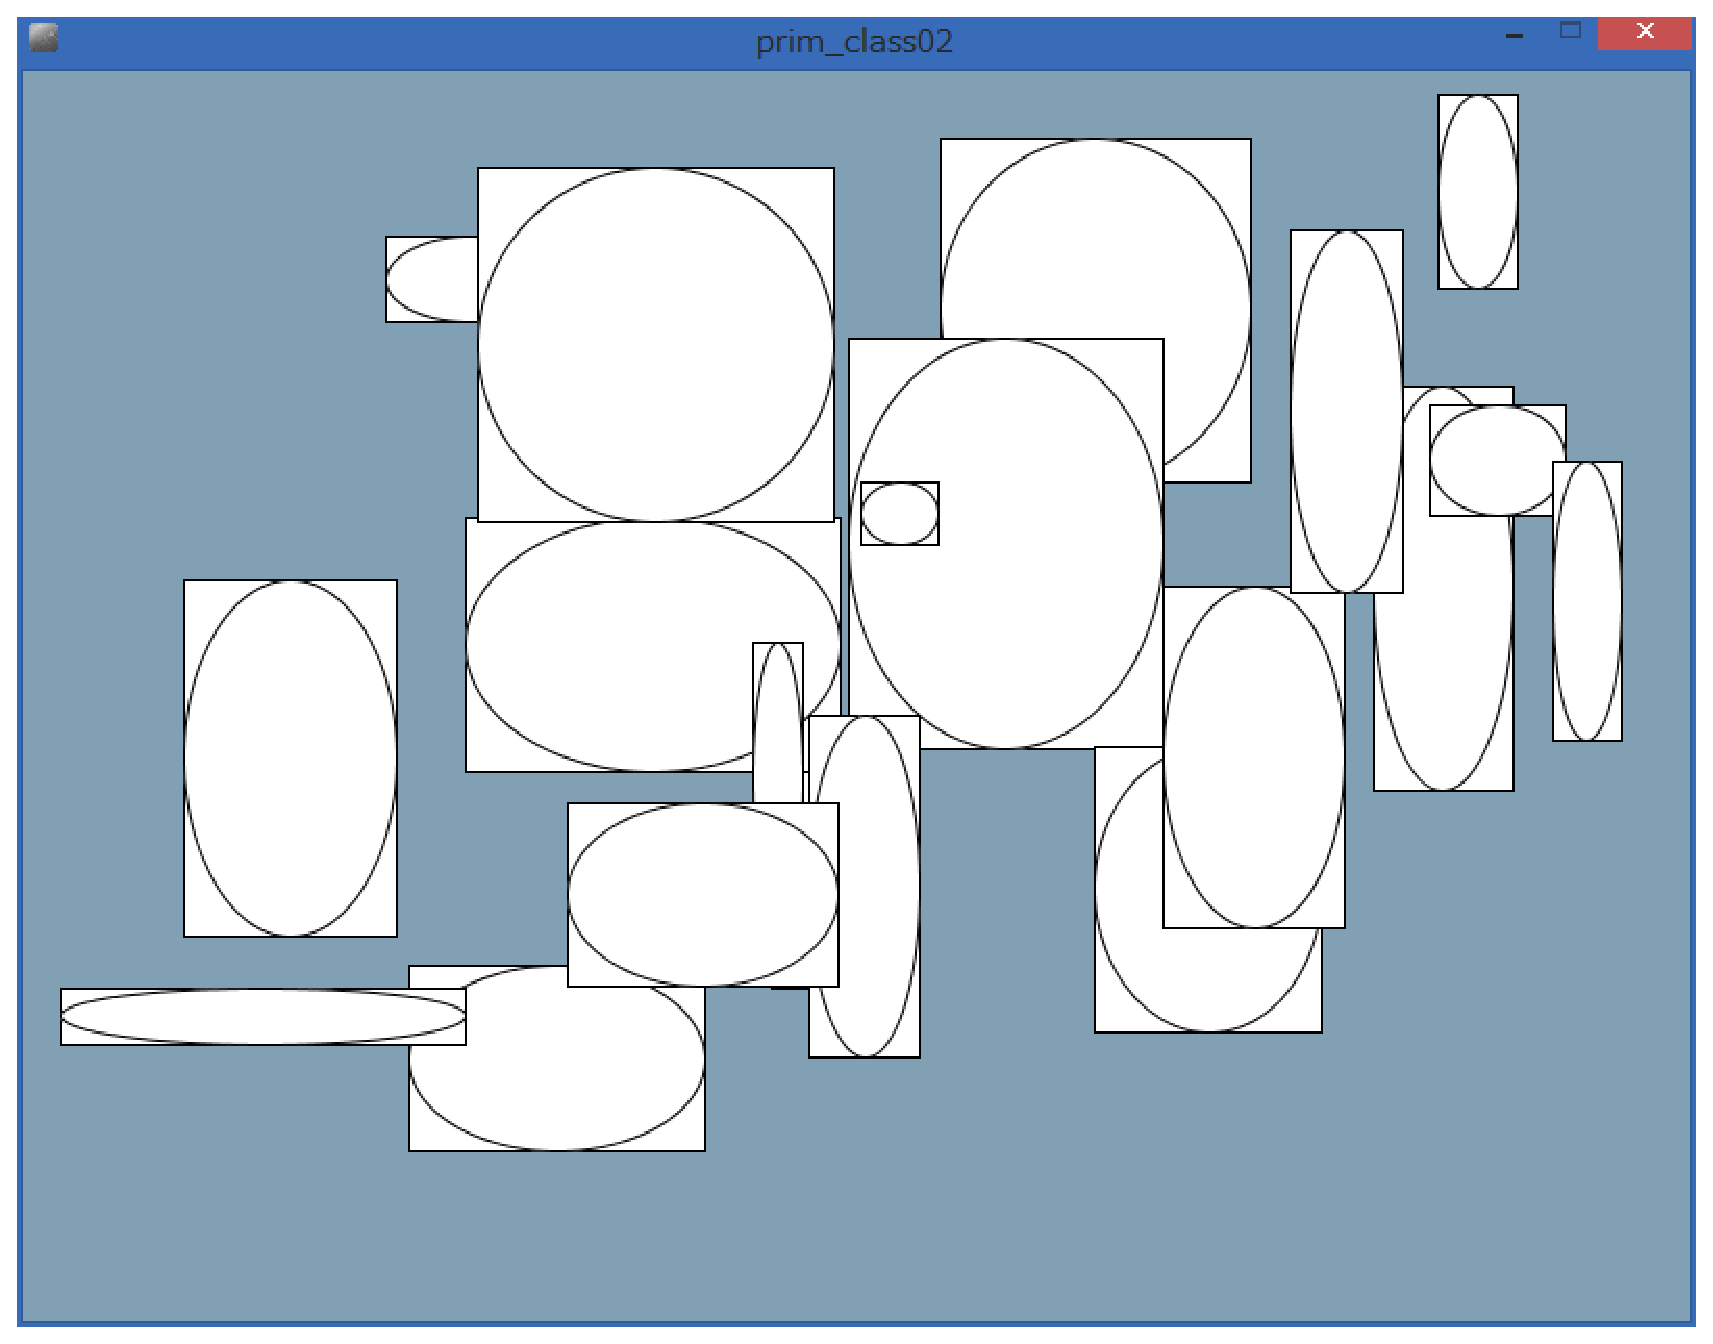
\includegraphics[width=.5\paperwidth]{zu3.eps}
   \caption{}
   \label{074547_20Jul14}
  \end{center}
\end{figure}

これは、

\begin{center}
 {\bfseries 四角が円を持つ (四角 has-a 円)}
\end{center}

ような形になっている。

四角が円を自分の中に取り込み、大きさを自分に合わせていると考えればよい。
これを{\bfseries 「has-a の関係」}または{\bfseries 「包含」}という。

四角クラスの中に円クラスのインスタンスを持つようにする。
円は四角の内部に取り込まれるので、外から見えるのは四角だけになる。
クラス図にすると図\ref{zu8}のようになる。

\begin{figure}[htbp]
 \begin{center}
   \includegraphics[width=.5\paperwidth]{zu10.eps}
   \caption{}
   \label{zu8}
 \end{center}
\end{figure}

\newpage
図\ref{zu8}では、次の点が変わっているを確認せよ。
\begin{itemize}
 \item カンバスから円クラス関連の属性・メソッドがなくなった
       \begin{itemize}
        \item 円は四角の中に隠蔽された、ということもできる
       \end{itemize}
 \item 四角クラスが円クラスのインスタンスを持つ\\
       ということは、以下の点が暗黙に了解される
       \begin{itemize}
        \item 「初期化する()」の中では円のインスタンスも初期化する
        \item 「描画する()」の中では円も同時に描画する
       \end{itemize}
 \item 円クラスに「データをセットする()」メソッドが追加された
       \begin{itemize}
        \item 四角の座標に合わせて円のデータ属性を書き換えるためのインター
              フェイスが必要になる。
       \end{itemize}
\end{itemize}

\href{prim_class02.txt}{コード例}

以前のコードにほんの数行の変更を加えるだけで、これらの動きが実現できた。
クラスにすると仕様変更が楽。これを最初にやっていたように、全ての図形を配
列にして処理していたとしたらどうだろうか?


\subsection{part-of の関係}

\subsubsection{(もう一度)共通点と相違点}

ここまでコーディングしてきた「四角クラス」と「円クラス」のソース・コード
を見比べてみよう。ほとんど同じコードになっている。それはそうだ。四角も円
も座標や大きさなど持っている属性は同じだし、図形を描く操作も同じだ。

違うのは具体的に四角を描いたり、円を描いたりする、最下層の proccessing
の関数の違いだけ。メソッドでいうと「\verb|drowPrim()|」の中身がちょっと
違うだけだ。

それなら、両方に共通する部分をまとめて書けないか?
とういうことで、もう一段階上の抽象的なクラスを新たに作ることを考える。

(複数あるオブジェクトの共通点を抜き出し、さらに上位の概念でまとめなおす
ことを「{\bfseries 抽象化}」という。その逆は「{\bfseries 具体化}」だ。)

四角と円の上位にある概念はなんだろう?

かくして「図形クラス」というものが、四角クラスと円クラスの上位概念として
見えてくる。

\begin{center}
 {\bfseries 四角と円は図形の一部である(四角 and 円 are part of 図形)}
\end{center}

というわけだ。

\href{prim_class20.txt}{コード例}

\subsection{継承}

クラス図にすると、図\ref{214654_21Jul14}のようになる。
四角クラスと円クラスが抽象化されて「図形クラス」が出来上がっているのが分
かるだろう。これを「{\bfseries 汎化}」という。

親クラスである「図形クラス」に、共通する属性と操作を組み込む。
子クラスでは親クラスの属性と操作を「{\bfseries 継承}」するので、改めて書
く必要はない。
書いてなくても、それらは子クラスにも存在するのだ。

\begin{figure}[htbp]
 \begin{center}
   \includegraphics[width=.4\paperwidth]{zu11.eps}
   \caption{}
  \label{214654_21Jul14}
 \end{center}
\end{figure}


\subsection{多態性}

一方、親クラスと異なる部分は、あらためて子クラスで定義することができる。

たとえば、図\ref{214654_21Jul14}の「\verb|drowPrim()|」は四角クラスと円
クラスで動きが違っているので、それぞれで中身を書く。
親クラスの「\verb|drowPrim()|」を子クラスで上書きして使うことになるので
「{\bfseries オーバーライド}」という。

すると「\verb|drowPrim()|」というメソッドは同じ名前でも、親クラスとそれ
を継承した子クラスとで振る舞いが違うことになる。

同じ名前なのに振る舞いが違うことを「{\bfseries 多態性(ポリモーフィズ
ム})」という。

C言語などでは同じ名前の関数が存在してはいけないので、このような場合次の
ように関数名を変更して混在させることになる。

\begin{itemize}
 \item drawPrimBox() : 四角を描く関数
 \item drawPrimCiecle() : 円を描く関数
\end{itemize}

これでも悪くはないが、「図形を描く」という、より抽象度の高いレベルで扱える
ことはシステムの設計には楽だ。

\section{抽象クラス}

「abstract」という指定子があってね...

「インターフェイス」とか「フレームワーク」とかに進んでいくんだけど、今の
ところはここまでにしておこうかな。

次のコード例は抽象クラスを使って書いてみた。

大きさと色も変化するように拡張してみた。
親クラスの中だけを書き換えればいいので楽だった。
こういう拡張性や保守性が、オブジェクト指向の目的である。
%\href{prim_class21.txt}{コード例}


    \begin{quote}
	\begin{minipage}{\linewidth}
	 \begin{shadebox}
      \def\baselinestretch{.8}\selectfont
      \small
      \begin{verbatim}
/*
 * 図形クラス prim_class20.pde
 *    CPrimを抽象クラスにした
 *    抽象クラスはnewでインスタンスを作成できない
 */
// abstract 指定
abstract class CPrim{
  // メンバ変数
  float x, y;  // 座標
  float w, h;  // 幅, 高さ  
  float moveX, moveY;  // 移動量
  float sizeW, sizeH;  // 大きさ変化量
  int colR, colG, colB;  // 色

  // コンストラクタ new でインスタンス(実体)が作られた時に
  // 最初に自動的に起動するメソッド
  CPrim(){
    //変数初期化
    x = random(width); y = random(height);
    w = random(10,200); h = random(10,200);
    moveX = random(1,10); moveY = random(1,10);
    // 位置調整
    if(x + w > width) x = width - (w + moveX);
    if(y + h > height) y = height - (h + moveY);
    sizeW = sizeH = 2;
    colR = int(random(256)); colG = int(random(256)); colB = int(random(256));
  }

  // 図形を描くメソッド
  // abstract なので抽象メソッドになる。
  // 中身は子クラスの方で定義する
  abstract void drawPrim();

  // 跳ね返りを判定するメソッド
  void checkDirection(){
    if(x < 0 || x + w + abs(sizeW) > width) moveX *= -1;
    if(y < 0 || y + h + abs(sizeH) > height) moveY *= -1;
    if(x + w  + abs(sizeW) > width) x -= abs(sizeW) + abs(moveX);
    if(y + h  + abs(sizeH) > height) y -= abs(sizeH) + abs(moveY);
  }

  // 大きさを変化するメソッド
  void cheangeSize(){
    if(w < 0 || w > 200) sizeW *= -1;
    if(h < 0 || h > 200) sizeH *= -1;
  }

  // 色を塗る
  void setColor(){
    colorMode(RGB,256);
    noStroke(); // 縁線を消す
    fill(colR, colG, colB);
    colR += 1; colG += 1; colB += 1;
    if(colR > 255) colR = 0;
    if(colG > 255) colG = 0;
    if(colB > 255) colB = 0;
  }
}
      \end{verbatim}
     \end{shadebox}
    \end{minipage}
    \end{quote}


    \begin{quote}
	\begin{minipage}{\linewidth}
	 \begin{shadebox}
      \def\baselinestretch{.8}\selectfont
      \small
      \begin{verbatim}
/*
 * 四角を描くクラス
 */
class CBox extends Prim{
  // 図形を描くメソッド
  void drawPrim(){
    setColor();
    rect(x, y, w, h);  // 四角を描く
    x += moveX; y += moveY;
    w += sizeW; h += sizeH;
    checkDirection();
    cheangeSize();
  }  
}

/*
 * 円を描くクラス
 */
class CCircle extends Prim{
  // 図形を描くメソッド
  void drawPrim(){
     setColor();
   // 円を描く
    ellipse(x + w / 2, y + h / 2, w, h);
    x += moveX; y += moveY;
    w += sizeW; h += sizeH;
    checkDirection();
    cheangeSize();
 }  
}

      \end{verbatim}
     \end{shadebox}
    \end{minipage}
    \end{quote}


『オブジェクト指向でなぜつくるのか』\cite{073146_20Jul14} には「クラスの
効能」として次の3点を挙げている。

\begin{quotation}
 クラスは「まとめて、隠して、たくさん作る」仕組み
 \begin{enumerate}
  \item サブルーチンと変数を「まとめる」
  \item クラスの内部だけで使う変数やサブルーチンを「隠す」
  \item 1つのクラスからインスタンスを「たくさん作る」
 \end{enumerate}
\end{quotation}

ここまでの実習で以上のことがわかってもらえたら幸いである。


% 参考文献
\begin{thebibliography}{99}
 \bibitem{Tucker}
         Tucker『憂鬱なプログラマのためのオブジェクト指向開発講座』 翔泳
         社, 1998
 \bibitem{073002_20Jul14}
         επιστημη『επιστημηのオブジェクト指向的日常』 翔泳
         社, 1999
 \bibitem{073146_20Jul14}
         平澤章『オブジェクト指向でなぜつくるのか 第2版』日経BP社, 2011
 \bibitem{073353_20Jul14}
         平澤章『UMLモデリングレッスン』日経BP社, 2013
\end{thebibliography}

\end{document}
%% ---------------------------------------------------------------


